\section{Results}

\textbf{Baseline.} Without perturbation SmolVLA succeeds in \BaseSpatial{} LIBERO-Spatial episodes
(10 tasks $\times$ 10) and in \BaseGoal{} LIBERO-Goal episodes. The Spatial rate is well below the 90\%
reported in~\citep{shukor2025smolvla}. To rule out our own evaluation loop, we re-ran two tasks with the
official \texttt{lerobot-eval}: \LerobotEvalCheck{}, against \OurEvalCheck{} with our loop on the same
tasks, a difference well within sampling noise. Two tasks (5 and 8) are solved in at most 2 of 10
episodes. All conclusions below are relative to this measured baseline.

\begin{figure*}[t]
  \centering
  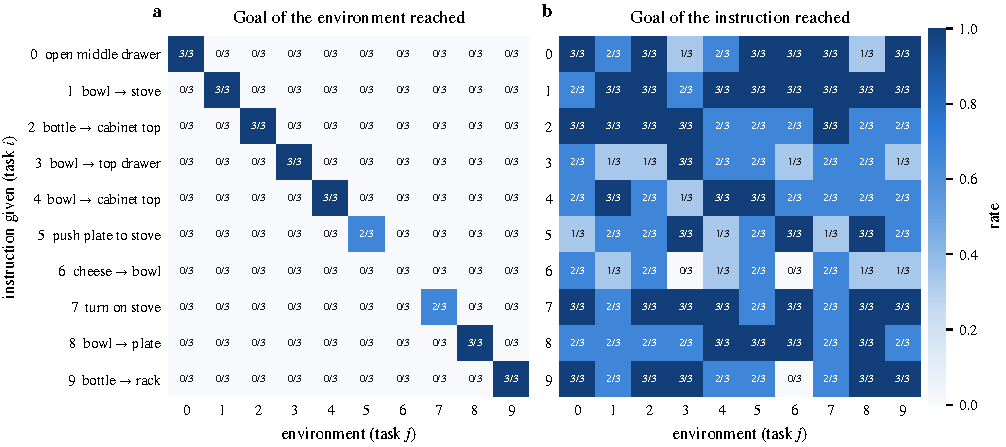
\includegraphics[width=\textwidth]{figures/language_matrix.pdf}
  \caption{\textbf{Listening test on LIBERO-Goal} (3 episodes per cell). The environment of task $j$ is
  built and the instruction of task $i$ is given. (a)~Success as scored by the environment (goal $j$).
  (b)~Whether the goal of the \emph{given} instruction $i$ was reached at any point of the episode,
  obtained by evaluating all ten goal predicates of the shared scene at every step. Off the diagonal
  the robot never completes the environment's own task, but reaches the instructed goal in
  \LangOffInstructedFrac{} of episodes.}
  \label{fig:language}
\end{figure*}

\subsection{SmolVLA follows the instruction}
Fig.~\ref{fig:language}a is the matrix one would get from the environment alone: success only on the
diagonal. Read in isolation it is ambiguous, since a robot that ignores language would also fail
off-diagonal if it performed some fixed behaviour unrelated to goal $j$. Panel~(b) removes the
ambiguity. When told to do task $i$ inside the environment of task $j$, the robot reaches goal $i$
in \LangOffInstructed{} of the 270 swapped episodes, close to the \LangDiag{} obtained with matched
instructions, and reaches the environment's goal in \LangOffEnvFrac{} of them; only \LangOther{}
episodes complete a third, unrelated goal. The initial states of the ten tasks differ slightly (each task
has its own set), so the robot is not keyed on the start configuration either. The weakest instructions
are those whose objects are close to other objects (task 3, bowl into the top drawer; task 6, cream
cheese into the bowl).

This contrasts with the conclusion of LIBERO-Plus that VLAs largely ignore language. The two tests
measure different things: paraphrases or corrupted instructions that do not change the intended goal
leave the action unchanged whether or not the model reads them, whereas swapping goals in a fixed
scene requires the instruction to be used. \LangVariantsSentence{}

\begin{figure*}[t]
  \centering
  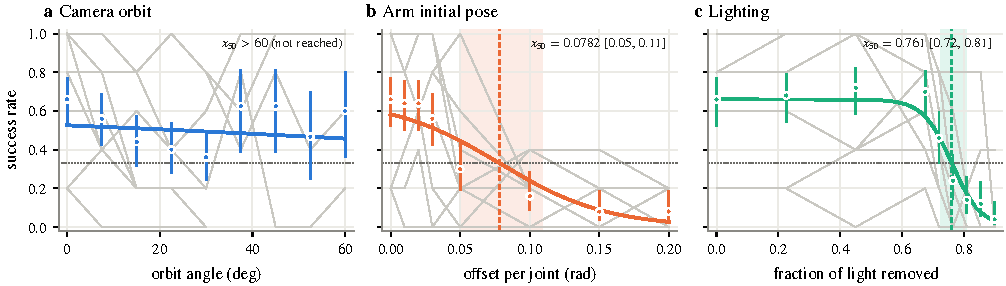
\includegraphics[width=\textwidth]{figures/dose_response.pdf}
  \caption{\textbf{Success versus perturbation intensity} on LIBERO-Spatial (10 tasks, 5 episodes per
  task and level; the unperturbed point uses the same episodes). Dots: pooled success with Wilson 95\%
  intervals. Grey: individual tasks. Line: logistic fit with $s_0$ fixed to the unperturbed rate; dotted:
  half of it. Dashed line and band: breaking point $x_{50}$ and its 95\% task-bootstrap interval.}
  \label{fig:dose}
\end{figure*}

\subsection{Three ways of breaking}
The perturbations do not just differ in strength; the curves have different shapes (Fig.~\ref{fig:dose}).
\begin{itemize}
  \item \textbf{Camera orbit: gradual.} Success declines roughly linearly with the angle and is halved at
  $x_{50}=\CamXfifty^\circ$ \CamXfiftyCI{}. The decline is strongly task dependent: some tasks are unaffected
  at the largest angle, others fail from the first level.
  \item \textbf{Arm initial pose: immediate.} An offset of \RobotXfifty{}\,rad per joint \RobotXfiftyCI{}
  halves success, although the wrist camera still sees the scene and the objects have not moved. This is
  the most sensitive axis by far relative to what a human would consider a meaningful change.
  \item \textbf{Lighting: threshold.} Removing up to two thirds of the light has no measurable effect; the
  policy then collapses between \LightCliffLow{} and \LightCliffHigh{} of light removed ($x_{50}=\LightXfifty$).
  Below the cliff the model is effectively invariant, which a single fixed-level test would miss
  entirely.
\end{itemize}
\NoiseSentence{}
\CameraMaskSentence{}

\begin{figure*}[t]
  \centering
  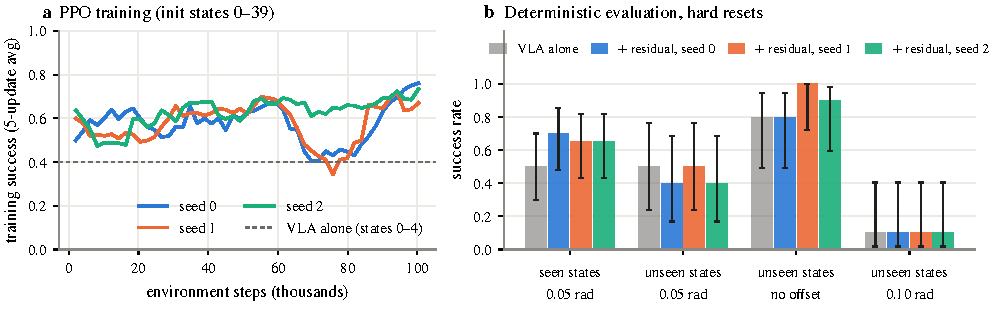
\includegraphics[width=\textwidth]{figures/rl_residual.pdf}
  \caption{\textbf{Residual RL on the arm-offset weakness} (LIBERO-Spatial task 2, offset 0.05\,rad per
  joint). (a)~Success of the stochastic policy during PPO, moving average over 5 updates (about 60
  episodes). (b)~Deterministic evaluation with hard resets, on initial states seen during training
  (0--19, 20 episodes) and on held-out ones (40--49, 10 episodes per bar). Wilson 95\% intervals.}
  \label{fig:rl}
\end{figure*}

\subsection{A residual corrector learns, but does not generalise}
\textbf{Target and design.} The arm-offset weakness is a natural target: the perturbation is visible in
proprioception, so a corrector without images can in principle detect it. We use LIBERO-Spatial task 2
at 0.05\,rad per joint, where the VLA alone succeeds in about half of the episodes. The corrector is an MLP
(two hidden layers of 128) that sees end-effector position and orientation, gripper opening, the VLA's
proposed action and the episode progress, and outputs $\Delta a\in[-1,1]^7$; the executed action is
$\mathrm{clip}(a_{\mathrm{VLA}} + 0.2\,\Delta a)$. Its last layer is initialised to zero, so before
training it reproduces the VLA exactly; we checked this on full episodes (identical outcomes and episode
lengths). It is trained with PPO~\citep{schulman2017ppo} in a single-file implementation in the style of
CleanRL~\citep{huang2022cleanrl}, with a sparse reward (1 on success), $\gamma=0.995$, four simulators in
one process sharing batched VLA calls, and 100k environment steps per run (about 400 episodes, 3\,h on
the laptop at 10 steps/s). Training uses initial states 0--39; states 40--49 are kept for evaluation.

\textbf{Results} (Fig.~\ref{fig:rl}). Training success rises modestly (from \RLTrainFirst{} to
\RLTrainLast{} over the first and last ten updates of each of the \RLSeeds{} seeds); seeds 0 and 1 dip around 70k steps before recovering, seed 2 does not. On initial states seen in training, the deterministic corrector succeeds in
\RLSeenRes{} episodes against \RLSeenVla{} for the VLA alone, and every discordant episode favours the
corrector (McNemar $p=$ \RLPSeen{}, not significant at this sample size). On held-out initial states the
gain disappears: \RLUnseenRes{} against \RLUnseenVla{} at the training level, \RLUnseenStrongRes{} against
\RLUnseenStrongVla{} at 0.10\,rad, and \RLUnseenCleanRes{} against \RLUnseenCleanVla{} without offset
(so the corrector does not hurt the unperturbed task).

What does transfer is speed: successful episodes are shorter with the corrector, from \RLStepsSeenVla{} to
\RLStepsSeenRes{} steps on seen states and from \RLStepsUnseenVla{} to \RLStepsUnseenRes{} on held-out
ones. This is what the objective rewards most directly: with discounting a faster success is worth more,
and speeding up an episode that already works is observed in every rollout, whereas recovering a failure
is a rare event in 400 episodes. The recoveries that do happen are tied to the configurations seen in
training; with 40 of them, the corrector has little to interpolate from.

A training-free alternative, executing 10 instead of 50 actions per chunk so that the VLA re-plans five
times more often, gives \RLReplanClean{}, \RLReplanTrain{} and \RLReplanStrong{} on the same held-out
episodes (no offset, 0.05 and 0.10\,rad), not distinguishable from the VLA alone with 10 episodes, at
\RLReplanSlowdown{}$\times$ the cost.

